\documentclass[a4paper,11pt]{article}

\usepackage[utf8]{inputenc}
\usepackage[T1]{fontenc}
\usepackage{mathptmx}

\usepackage[a4paper,text={160mm,220mm},centering]{geometry}

\usepackage{hyperref}
\usepackage{listings}
\usepackage{graphicx}
\usepackage[table]{xcolor}

\lstset{basicstyle={\ttfamily}}

\begin{document}


\unitlength=1mm
\begin{picture}(0,0)(0,10)
\put(-20,25){
\includegraphics[width=0.3\textwidth]{../images/Logo_Bpifrance.png}
  
\includegraphics[width=0.1\textwidth]{../images/Logo-France-2030-rouge-bleu.png}}
\end{picture}

\begin{center}\bfseries

  \Huge
  Projet Décysif --- Livrable 2.1

  \Large
Constitution d’une base de fichiers d’entrée
représentatifs des difficultés rencontrées pour la
preuve automatique.
\end{center}


Ce livrable est constituée d'une base de tests qui se trouve dans le dépot
\href{https://github.com/Decysif/benchmarks}{'benchmarks'} du projet Décysif.

Objectifs du livrable :

\begin{itemize}
\item Repérer les faiblesses du prouveur Alt-Ergo
\item Repérer les problèmes de traduction (ou repérer des problèmes au niveau de l'écriture des théories, par exemple le modèle mémoire de J3) pour tous les prouveurs cvc5, CVC4, Z3, Alt-Ergo.
\end{itemize}

% Une section par répertoire d'exemples avec une description du contenu
% et de la méthodologie des statisques adoptée. Et le résultat de ces statisques
% au démarrage du projet.

% Mettre les statistiques qu'on a quand elles existent.

\section{Examples issus de Why3}

Le sous-répertoire \url{why3_examples} contient le jeu d'exemples
extrait du bench complet de Why3, formé de code source dans le langage
WhyML. La documentation de référence est dans le fichier \url{README.md} de ce répertoire.
Pour installer et configurer ce jeu de tests, la commande
\begin{lstlisting}
> ./import_suite.sh
\end{lstlisting}
doit être exécutée au préalable. Ceci récupère une version de
référence de Why3 (1er mars 2024) et compile les commandes nécessaires. Ensuite la commande
\begin{lstlisting}
> ./run_bench.sh
\end{lstlisting}
pour être lancée pour executer les tests proprement dit. Les prouveurs
utilisés pour ces tests sont indiqués dans le fichier
\url{run_bench.sh} lui-même.

Une exécution de référence de ces tests a été lancée le 15 avril 2024
sur le serveur de calcul ``moloch'' de l'équipe Inria Toccata. Ce
serveur dispose de 16 c{\oe}urs ``Intel(R) Xeon(R) CPU E5-2450 v2 @
2.50GHz'' et de 64 Go de memoire centrale. Pour ces tests, 8 c{\oe}urs
ont été utilisés. Sur chaque fichier source, on demande à Why3 de
générer l'obligation de preuve de chaque fonction, de découper la
formule générée en plusieurs sous-formules, puis on appelle un jeu de
prouveur sur chacune des sous-formules. Un temps limite de 5 secondes est donné à chaque exécution de prouveurs. Pour l'exécution de référence,
les prouveurs Alt-Ergo 2.5.2, CVC4 1.8, cvc5 1.0.5 et Z3 4.12.2 ont
été utilisés. Les résultats sont enregistrés dans des fichiers de
session de preuve de Why3, pouvant donner lieu à diverses
statistiques. Voici des statistiques globales pour l'exécution de
référence, le nombre total d'obligation de preuve est de 41389:
\begin{center}
  \rowcolors{2}{gray!25}{white}
  \begin{tabular}{|l|r|r|r|r|r|}
  \rowcolor{gray!50} Prouveur
  & \multicolumn{1}{p{0.13\textwidth}|}{nombre de but prouvés }
  & \multicolumn{1}{p{0.13\textwidth}|}{nombre de buts}
  & \multicolumn{1}{p{0.13\textwidth}|}{temps minimal}
  & \multicolumn{1}{p{0.13\textwidth}|}{temps maximal}
  & \multicolumn{1}{p{0.13\textwidth}|}{temps moyen}
  \\
  Alt-Ergo 2.5.2                & 41389 & 32170 &  0.00  & 4.98 &  0.12 \\
  CVC4 1.8                      & 41389 & 33650 &  0.01  & 4.81 &  0.17 \\
  CVC5 1.0.5                    & 41389 & 32904 &  0.01  & 4.92 &  0.17 \\
  Z3 4.12.2                     & 41389 & 30713 &  0.01  & 4.96 &  0.07
\end{tabular}
\end{center}

\begin{figure}
  \centering
  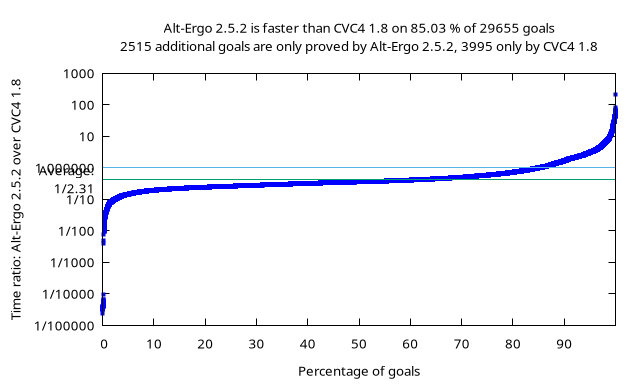
\includegraphics[width=0.9\textwidth]{AE-vs-CVC4.png}
  \caption{Comparaison d'Alt-Ergo et CVC4. Globalement, CVC4 prouve
    plus de buts qu'Alt-Ergo, mais Alt-Ergo est plus rapide. On
    indique aussi que 2515 buts sont prouvés par Alt-Ergo mais pas par
    CVC4, alors que 3995 sont prouvés par CVC4 mais pas par Alt-Ergo.}
  \label{fig:AEvsCVC4}
\end{figure}

Des statistiques plus fines peuvent être calculées à la demande sur
les fichiers de sessions. Par exemple, la figure~\ref{fig:AEvsCVC4}
une représentation graphique qui compare les performances de Alt-Ergo
et de CVC4 sur le jeu de test.

En fin de projet, une exécution similaire des outils améliorés seront
rejoués sur les même exemples, et on évaluera les améliorations
apportées en terme de pourcentage de preuve automatique réussies.


\section{Examples issus de J3}

TODO [Guillaume]

Méthodologie pour extraire des statistique à décrire:
* Nombre de buts prouvés/Nombre de buts au total
TODO: Fixer la version d'alt-ergo

\section{Examples issus de SPARK}

TODO [Yannick]

\section{Examples issus de Creusot}

TODO [Claude]

\section{Travail futur}

Quelles autres statistiques peut-on vouloir?

\end{document}
